\newpage
\subsection{Lineare Funktionen mit 2 Variablen}

Jede lineare Gleichung lässt sich auf eine Faktorgleichung der Form $y=kx+d$ umformen.
$$ax+by = c$$
$$\downarrow$$
$$y=\frac{c-ax}{b}$$

\hfill \break
Example:\\
\fboxrule=0.8pt \fcolorbox{black}{lightgray}{%
    \begin{tabular}[t]{@{}l@{}}
        $x+y=5$ /-x \\
        $y=5-x$     \\
        $y=-x+5$    \\
        $y=-1x+5$   \\
    \end{tabular}}
\begin{itemize}
    \item $d=5$
    \item $k=-1$
\end{itemize}

\hfill \break
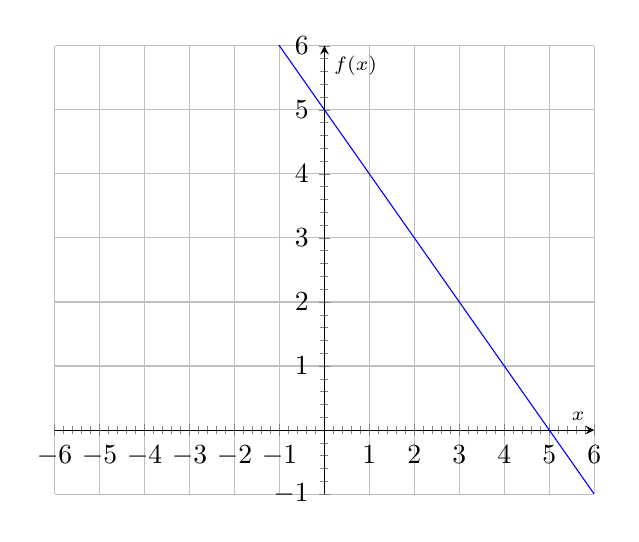
\begin{tikzpicture}[scale=1.0]
    \begin{axis}%
        [
            grid=major,
            xtick={-7,-6,...,7},
            minor x tick num=4, % 4 minor ticks => 5 subintervals
            xmin=-6,
            xmax=6,
            xlabel={\scriptsize $x$},
            axis x line=middle,
            ytick={-5,-4,...,6},
            minor y tick num=4,  % 4 minor ticks => 5 subintervals
            ymin=-1,
            ymax=6,
            ylabel={\scriptsize $f(x)$},
            axis y line=middle,
            no markers,
            samples=100,
            domain=-6:6,
        ]
        \addplot (x,{-1*x+5});
    \end{axis}
\end{tikzpicture}

\hfill \break
Lösungsverfahren:
\begin{itemize}
    \item Graphisch
    \item Rechnerisches Gleichsetzungsverfahren
    \item Rechnerisches Einsetzungsverfahren
    \item Rechnerisches Eliminationsverfahren
\end{itemize}

\break
\newpage
\subsubsection{Gleichsetzungsverfahren}

Beim Gleichsetzungsverfahren werden beide Terme Gleichgesetzt.

\hfill \break
Example:\\
\fboxrule=0.8pt \fcolorbox{black}{lightgray}{%
    \begin{tabular}[t]{@{}l@{}}
        (1):$y=x+1 $ / $y=2$   \\
        (2):$y=-2x+4 $ / $y=2$ \\
        \\
        \\
        $y_1 = y_2$            \\
        $x+1 = -2x+4$ /+2x     \\
        $3x+1 = 4$ /-1         \\
        $3x = 3$ / /3          \\
        $x = 1$                \\
    \end{tabular}}

$$L=\{1,2\}$$
\break
\subsubsection{Einsezuungsverfahren}

Beim Einsezuungsverfahren wird ein Term in den anderen eingesetzt.

\hfill \break
Example:\\
\fboxrule=0.8pt \fcolorbox{black}{lightgray}{%
    \begin{tabular}[t]{@{}l@{}}
        (1):$y=x+1$                                  \\
        (2):$+2x+y=4$ / $x+1$ wird in $y$ eingesetzt \\
        \\
        \\
        $+2x+x+1 = 4$                                \\
        $3x+1 = 4$ / -1                              \\
        $3x = 3$ / /3                                \\
        $x = 1$                                      \\
    \end{tabular}}

$$L=\{1,2\}$$
\break
\newpage
\subsubsection{Eliminationsverfahren}

Beim Eliminationsverfahren wird ein Teil des ersten Termes vom zweiten Term subtrahiert.

\hfill \break
Example:\\
\fboxrule=0.8pt \fcolorbox{black}{lightgray}{%
    \begin{tabular}[t]{@{}l@{}}
        (1):$y=x+1$ /$y$ wird elemeniert   \\
        (2):$y=-2x+4$ /$y$ wird elemeniert \\
        \\
        \\
        $0=x-(-2x)+1-4$                    \\
        $0=x+2x-3$                         \\
        $3=3x$ / /3                        \\
        $1=x$                              \\
    \end{tabular}}

$$L=\{1,2\}$$

\hfill \break
Um $x$ elemenieren zu können muss man zuerst bei beide Gleichungen die selbe Anzahl an $x$ erzeugen.

\hfill \break
Example:\\
\fboxrule=0.8pt \fcolorbox{black}{lightgray}{%
    \begin{tabular}[t]{@{}l@{}}
        (1):$4x + y = 16$          \\
        (2):$4x - 2y  = - 8 $ / /2 \\
        (2):$2x - y  = - 4$        \\
        \\
        \\
        $4x+y=16$                  \\
        $2x-y=-4$                  \\
        $6x=12$                    \\
        $x=2$                      \\
        \\
        \\
        In Ursprungsform Einsetzen \\
        $4*2+y=16$                 \\
        $8+y=16$ / -8              \\
        $y=8$                      \\
    \end{tabular}}

$$L=\{2,8\}$$
\newpage
\subsubsection{Sonderfälle}

\hfill \break
Example 1.Sonderfall:\\
\fboxrule=0.8pt \fcolorbox{black}{lightgray}{%
    \begin{tabular}[t]{@{}l@{}}
        (1):$3x+2y=4$ / *2 \\
        (2):$-6x-4y=-8$    \\
        (1):$6x+4y=8$      \\
        \\
        \\
        $0+0 = 0$          \\
        $0 = 0$            \\
    \end{tabular}}\\

\hfill \break
Example 2.Sonderfall:\\
\fboxrule=0.8pt \fcolorbox{black}{lightgray}{%
    \begin{tabular}[t]{@{}l@{}}
        (1):$3x+2y=4$ / *3 \\
        (2):$9x+6y=10$     \\
        (1):$9x+6y=12$     \\
        \\
        \\
        $0+0 = 2$          \\
        $0 = 2$ / $f.A$    \\
    \end{tabular}}\\